\documentclass[12pt]{article}
\usepackage{amsmath}
\usepackage{graphicx}
\usepackage{caption}
\usepackage{subcaption}
\usepackage{booktabs}
\usepackage{float}
\usepackage[utf8]{inputenc}
\usepackage{geometry}
\usepackage{multirow}
\usepackage{setspace}
\usepackage{parskip}
\usepackage{svg}
\usepackage[bottom]{footmisc}
\usepackage{tikz}
\usepackage[section]{placeins}

% This style is used to create block diagrams, you'll find it useful since many of your figures would be of that form, I'll try add more styles in the future :)
\usetikzlibrary{trees,positioning,fit,calc}
\tikzset{block/.style = {draw, fill=blue!20, rectangle,
                         minimum height=3em, minimum width=4em},
        input/.style = {coordinate},
        output/.style = {coordinate}
}

\usepackage[section]{minted}
\usepackage{xcolor}
\usemintedstyle{porland}

\usepackage{chngcntr}
\counterwithin{figure}{section}

\renewcommand{\arraystretch}{1.5}

\usepackage[hidelinks]{hyperref}
\hypersetup{
    linktoc=all
}

\renewcommand\listingscaption{Listing}
\renewcommand\listoflistingscaption{List of Listings}

\usepackage{scrhack}
\usepackage{tocbasic}
\setuptoc{lol}{levelup}

\usepackage{indentfirst}
\geometry{a4paper, margin=1in}

%----------EDIT COVER INFO HERE -----------------%

\def \DEPARTEMENT {Department of Computer Science }
\def \COURSENUM {COSC 4P80}
\def \COURSENAME {Artificial Neural Network}
\def \REPORTTITLE {Bidirectional Associative Memory - BAM}
\def \STUDENTNAME {Hridoy Rahman}
\def \STUDENTID {7340334}
\def \INSTRUCTOR {Dave Bockus}

%------------------------------------------------%

\setlength{\parindent}{0em}
\setlength{\parskip}{0em}

\begin{document}

\pagenumbering{Roman}

\begin{titlepage}
    \vfill
    \begin{center}
        \hfill \\
        \Large{\DEPARTEMENT} \\
        \Large{\COURSENUM\;-\;\COURSENAME} \\
        \vfill
        \textbf{\LARGE{\REPORTTITLE}}
    \end{center}
    \vfill
    \begin{flushleft}
        \Large{\textbf{Prepared by:} \STUDENTNAME} \\
        \Large{\textbf{Instructor:} \INSTRUCTOR} \\
        \Large{\textbf{Date:} \today}
    \end{flushleft}
    \vfill
\end{titlepage}

%--------------ABSTRACT ------------------------%
{
\centering
\section*{Abstract}
Bidirectional Associative Memory is a type of recurrent neural network that uses associative memory. Associative memory stores associations between patterns and recalls a pattern when presented with another pattern. The assignment is related to BAM Networks, and for part A of the Assignment, a BAM Network is created where the network can take an input pattern and return an associated pattern.
On the contrary, if an output pattern is given, it can also recall its input pattern association. The second part of the assignment is based on cross-talk of the Input vector set A. If the input vectors are not orthogonal, the response will include a portion of their target values. This is called the cross talk. For part(B), the cross-talk calculation of vector input set A is provided. In part(C), the input vector set A is extended with the provided example vector, and three more are added randomly. Then, the crosstalk calculation for extended vector set A is provided in part(C).
Additionally, in part(D), a small experiment is done, including mutating the original input vector set A with a 20\% mutation rate. Then, the BAM network is applied to error-correct the mutated input vector set. Following that, a table is formulated to show the runs, original vector listings, and mutated vector set listing, the hamming distance, the corrected vector set and the hamming distance between the original and error-corrected vector set. Finally, this report concludes with the learning of the experiments done in this assignment.

\clearpage
}

%-----------------------------------------------%

\tableofcontents
\clearpage

\setlength{\parskip}{\baselineskip}%

\pagenumbering{arabic}

%--------------INTRODUCTION ---------------------%

\section{Introduction}

\subsection{BAM Network}
Bidirectional Associative Memory is a type of recurrent neural network that works using associative memory. Associative memory stores associations between patterns and recalls a pattern when presented with another pattern. BAM is a hetero-associative network that takes two different input and output sets to learn patterns. In other words, given an input pattern, BAM can retrieve another pattern of a different size. For example, take a vector from the input set A [1,-1,1,-1]. If the network is trained properly, then the BAM network will return a pattern [1, 1, -1, 1, 1] that is associated with the given input. This section exhibits a created BAM Network where the network can take an input pattern and return an associated pattern. On the contrary, if an output pattern is given, it can also recall its input pattern association. For example, Diagram 1 shows that an input vector is multiplied with a 
transposed weight matrix to recall the output pattern associated with the input vector. Inversely, if an output vector is multiplied by the matrix, the associated input pattern with the output vector is returned(Diagram 2). A weight matrix is needed to achieve this BAM network, which helps store the association between input and output patterns. The weight matrix is achieved by applying the following formula: w. 

\[
\text{Weight Matrix, }
w = \sum_{k=1}^{m} A_k B_k^T
\]
\[
A = \begin{bmatrix}
-1 & 1 & 1 & 1 & -1 \\
-1 & -1 & -1 & -1 & 1 \\
-1 & -1 & -1 & 1 & 1 
\end{bmatrix}
\]

\[
B^T = \begin{bmatrix}
1 & 1 & -1 & 1 \\
1 & -1 & -1 & -1 \\
-1 & -1 & 1 & 1 
\end{bmatrix}
\]
Now, we can calculate \( w \) using the formula:
Where:
- \( A_k \) is a row from matrix \( A \).
- \( B_k \) is a row from matrix \( B \).
This results in the following calculations:
\[
\begin{aligned}
w &= A_1 B_1^T + A_2 B_2^T + A_3 B_3^T \\
  &= \begin{bmatrix}
-1 & 1 & 1 & 1 & -1 
\end{bmatrix}
\begin{bmatrix}
1 \\
1 \\
-1 \\
1 
\end{bmatrix}
+
\begin{bmatrix}
-1 & -1 & -1 & -1 & 1 
\end{bmatrix}
\begin{bmatrix}
1 \\
-1 \\
-1 \\
-1 
\end{bmatrix}
+
\begin{bmatrix}
-1 & -1 & -1 & 1 & 1 
\end{bmatrix}
\begin{bmatrix}
-1 \\
-1 \\
1 \\
1 
\end{bmatrix}
\end{aligned}
\]

The above formula, w shows the formula to calculate the weight matrix. \\

Here, in diagram, a vector input is multiplied with the weight matrix and an associated output vector is provided back. Which shows the association between X to Y. 
\[
\begin{bmatrix}
-1 & 1 & 1 & 1 & -1
\end{bmatrix}
\begin{bmatrix}
-1 &  1 &  1 & -1 & -1 \\
 1 &  3 &  3 &  1 & -3 \\
 1 & -1 & -1 &  1 &  1 \\
 -1 &  1 &  1 &  3 & -1 \\
\end{bmatrix}
=
\begin{bmatrix}
1 & 1 & -1 & 1
\end{bmatrix}
\]
\[
\text{Diagram 1: } X \cdot W^T = Y
\]

On the contrary, in this following diagram, an output vector is multiplied with the weight matrix, which results back the input pattern associated with the output which in this case is the input to the BAM Network. Here, the associations shows that, Y -> X is also possible. 
\[
\begin{bmatrix}
1 & 1 & -1 & 1
\end{bmatrix}
\begin{bmatrix}
-1 &  1 &  1 & -1 \\
 1 &  3 & -1 &  1 \\
 1 &  3 & -1 &  1 \\
-1 &  1 &  1 &  3 \\
-1 & -3 &  1 & -1 \\
\end{bmatrix}
=
\begin{bmatrix}
-1 & 1 & 1 & 1 & -1
\end{bmatrix}
\]

\[
\text{Diagram 2: } Y \cdot W = X
\]

In the following Experiment and Result section, A set of inputs will be provided to an implemented BAM network, following that the result will be provided by emphasizing whether the BAM network recalled properly or not. The second experimental part will include the cross-talk of the Input vectors, The results should contain the calculation table of the cross-talk. Third experiment includes inserting new pairs to the BAM network and retrain the BAM model and showing the generated inference once again by checking the cross talk of the input vectors in terms of the output vectors as well as to show that the network will saturate at one point, will not recall correctly, and cross-talk increases. The Part four, includes an experiment where the original input vectors are mutated with 20\% probability and then the hamming distance of original, mutated vectors are calculated. Additionally, for the result, a table is provided showing all the required outputs and a discussion of it.

\break

\subsection{Part(A)}

After creating a BAM network, provided two input vector A, B is used as the input for the BAM Network.
The output of the BAM Network is shown in Table 1 and Table 2. Table 1 shows the result for A vector set is given to BAM network as input and the BAM model predicted the Output for each associated input vector in set A. Table 2 shows that the BAM network takes B vector set as input and it predicts the input vectors associated with each output vector in B.

\begin{table}[ht]
    \centering
    \caption{Results of A to B Mappings}
    \begin{tabular}{|c|c|c|c|}
        \hline
        \textbf{Input} & \textbf{Target} & \textbf{Output} & \textbf{Result} \\ \hline
        $A = [-1, 1, 1, 1, -1]$ & $[1, 1, -1, 1]$ & $[1, 1, -1, 1]$ & True \\ \hline
        $A = [-1, -1, -1, -1, 1]$ & $[1, -1, -1, -1]$ & $[-1, -1, 1, -1]$ & False \\ \hline
        $A = [-1, -1, -1, 1, 1]$ & $[-1, -1, 1, 1]$ & $[-1, -1, 1, 1]$ & True \\ \hline
    \end{tabular}
\end{table}

\vspace{1cm} % Adds vertical space between the tables

\begin{table}[ht]
    \centering
    \caption{Results of B to A Mappings}
    \begin{tabular}{|c|c|c|c|}
        \hline
        \textbf{Input} & \textbf{Target} & \textbf{Output} & \textbf{Result} \\ \hline
        $B = [1, 1, -1, 1]$ & $[-1, 1, 1, 1, -1]$ & $[-1, 1, 1, 1, -1]$ & True \\ \hline
        $B = [1, -1, -1, -1]$ & $[-1, -1, -1, -1, 1]$ & $[1, -1, -1, -1, 1]$ & False \\ \hline
        $B = [-1, -1, 1, 1]$ & $[-1, -1, -1, 1, 1]$ & $[1, -1, -1, -1, 1]$ & False \\ \hline
    \end{tabular}
\end{table}

From the output tables, it is visible that 3 of the predictions were false. Which means the BAM network didn't recall properly. The reason is because of the activation function. The activation function for from A to B is the same as the activation function for from B to A. Which made the model predict inaccurately. With an improved activation function it is possible to improve the BAM models output. In the above table 1 and table 2, follows the below activation function. 
\vspace{-1cm}
\begin{center}
\[
b_j(t+1) = 
\begin{cases} 
1 & \text{if } y_j > 0 \\ 
b_j(t) & \text{if } y_j = 0 \\ 
-1 & \text{if } y_j < 0 
\end{cases}
\]
\end{center}
This activation function is applied for A vectors to predict B vectors and B vector set to predict A vector set. Meaning, A vector set used for predicting B output vectors, and vice versa. 

However, if the activation function from B to A is changed then the results improves. 

\[
\text{activationFunction1}(y) = 
\begin{cases} 
1 & \text{if } y \geq 0 \\ 
-1 & \text{if } y < 0 
\end{cases}
\]

The following threshold function, activateFunction1 is used for forward activation, meaning using vector A set to predict the vector B set. And activateFunction2 is used for backward activation meaning vector B set is used as input for the BAM and the input vector set A is predicted by the model.

\[
\text{activationFunction2}(x) = 
\begin{cases} 
-1 & \text{if } x \leq 0 \\ 
1 & \text{if } x > 0 
\end{cases}
\]

\begin{table}[ht]
    \centering
    \caption{Results of A to B Mappings}
    \begin{tabular}{|c|c|c|c|}
        \hline
        \textbf{Input} & \textbf{Target} & \textbf{Output} & \textbf{Result} \\ \hline
        $A = [-1, 1, 1, 1, -1]$ & $[1, 1, -1, 1]$ & $[1, 1, -1, 1]$ & True \\ \hline
        $A = [-1, -1, -1, -1, 1]$ & $[1, -1, -1, -1]$ & $[-1, -1, 1, -1]$ & False \\ \hline
        $A = [-1, -1, -1, 1, 1]$ & $[-1, -1, 1, 1]$ & $[-1, -1, 1, 1]$ & True \\ \hline
    \end{tabular}
\end{table}

\begin{table}[ht]
    \centering
    \caption{Results of B to A Mappings}
    \begin{tabular}{|c|c|c|c|}
        \hline
        \textbf{Input} & \textbf{Target} & \textbf{Output} & \textbf{Result} \\ \hline
        $B = [1, 1, -1, 1]$ & $[-1, 1, 1, 1, -1]$ & $[-1, 1, 1, 1, -1]$ & True \\ \hline
        $B = [1, -1, -1, -1]$ & $[-1, -1, -1, -1, 1]$ & $[1, -1, -1, -1, 1]$ & False \\ \hline
        $B = [-1, -1, 1, 1]$ & $[-1, -1, -1, 1, 1]$ & $[-1, -1, -1, 1, 1]$ & True \\ \hline
    \end{tabular}
\end{table}

From the Table 3 and Table 4, it is visible that it indeed improves the results by changing the threshold function. 

Furthermore, if the cross-talk interference is too much between two pattern set then it is possible for the similar stored patterns to lead to false recalls. 

\break
\subsection{Part(B)}
The Cross-talk Calculation of Vector Set A:

\begin{table}[ht]
    \centering
    \caption{Vectors \( A \) and \( B \)}
    \begin{tabular}{|c|c|}
        \hline
        \textbf{Input Vector \( A \)} & \textbf{Output Vector \( B \)} \\ \hline
        $[-1, 1, 1, 1, -1]$ & $[1, 1, -1, 1]$ \\ \hline
        $[-1, -1, -1, -1, 1]$ & $[1, -1, -1, -1]$ \\ \hline
        $[-1, -1, -1, 1, 1]$ & $[-1, -1, 1, 1]$ \\ \hline
    \end{tabular}
\end{table}

And the magnitude of each vector ${C_i}$ is given below,

\begin{figure}[ht]
    \centering
    \begin{minipage}{0.45\textwidth}
        \centering
        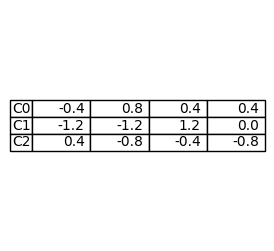
\includegraphics[width=\linewidth]{CrossTalk.png}
        \caption{Cross Talk of Vectors}
        \label{fig:crosstalk}
    \end{minipage}\hfill
    \begin{minipage}{0.45\textwidth}
        \centering
        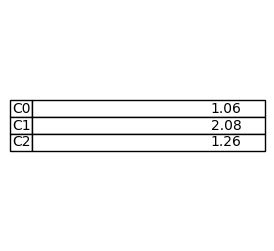
\includegraphics[width=\linewidth]{magnitude.png}
        \caption{Magnitude of Vectors}
        \label{fig:magnitude}
    \end{minipage}
\end{figure}

\break

\subsection{Part(C)}
\begin{table}[ht]
    \centering
    \caption{Vectors \( A \) and \( B \)}
    \begin{tabular}{|c|c|}
        \hline
        \textbf{Input Vector \( S \)} & \textbf{Output Vector \( T \)} \\ \hline
        $[-1, 1, 1, 1, -1]$ & $[1, 1, -1, 1]$ \\ \hline
        $[-1, -1, -1, -1, 1]$ & $[1, -1, -1, -1]$ \\ \hline
        $[-1, -1, -1, 1, 1]$ & $[-1, -1, 1, 1]$ \\ \hline
        $[1, 1, 1, 1, 1]$ & $[-1, 1, 1, -1]$ \\ \hline
    \end{tabular}
\end{table}

The output after adding the new pair provided in the assignment, the output of the BAM network is provided below, 

\begin{table}[ht]
    \centering
    \caption{Predictions from \( A \) to \( B \)}
    \begin{tabular}{|c|c|c|c|c|}
        \hline
        \textbf{Input \( x \)} & \textbf{Target} & \textbf{Predicted Output \( y \)} & \textbf{Result} \\ \hline
        $[-1, 1, 1, 1, -1]$ & $[1, 1, -1, 1]$ & $[1, 1, -1, 1]$ & True \\ \hline
        $[-1, -1, -1, -1, 1]$ & $[1, -1, -1, -1]$ & $[1, -1, -1, 1]$ & False \\ \hline
        $[-1, -1, -1, 1, 1]$ & $[-1, -1, 1, 1]$ & $[-1, -1, 1, 1]$ & True \\ \hline
        $[1, 1, 1, 1, 1]$ & $[-1, 1, 1, -1]$ & $[-1, 1, 1, -1]$ & True \\ \hline
    \end{tabular}
\end{table}

\vspace{1cm} % Adds vertical space between the tables

\begin{table}[ht]
    \centering
    \caption{Predictions from \( B \) to \( A \)}
    \begin{tabular}{|c|c|c|c|c|}
        \hline
        \textbf{Output \( y \)} & \textbf{Target} & \textbf{Predicted Output \( x \)} & \textbf{Result} \\ \hline
        $[1, 1, -1, 1]$ & $[-1, 1, 1, 1, -1]$ & $[-1, 1, 1, 0, -1]$ & False \\ \hline
        $[1, -1, -1, -1]$ & $[-1, -1, -1, -1, 1]$ & $[-1, -1, -1, -1, -1]$ & False \\ \hline
        $[-1, -1, 1, 1]$ & $[-1, -1, -1, 1, 1]$ & $[1, -1, -1, 0, 1]$ & False \\ \hline
        $[-1, 1, 1, -1]$ & $[1, 1, 1, 1, 1]$ & $[1, 1, 1, 1, 1]$ & True \\ \hline
    \end{tabular}
\end{table}

After adding one more vector to the BAM model, the model starts predicting more inaccurately. That is because of too much of cross talk between two pairs of vectors increased. Note that, vector magnitude in figure 1.4, shows an increase in magnitude in terms of magnitude shown in figure 1.2. In figure 1.2, vector C0 and vector C2's cross talk increased in figure 1.4, which means after adding one more vector to the BAM model. Now, showing the cross-talk calculation of the new vector pairs. And the magnitude of each vector ${C_i}$ is given below,

\begin{figure}[ht]
    \centering
    \begin{minipage}{0.45\textwidth}
        \centering
        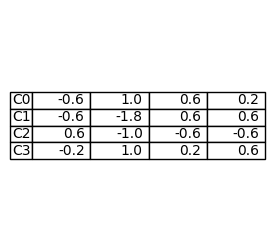
\includegraphics[width=\linewidth]{CrossTalk2.png}
        \vspace{-2cm}
        \caption{Cross Talk of Vectors}
        \label{fig:crosstalk}
    \end{minipage}\hfill
    \begin{minipage}{0.45\textwidth}
        \centering
        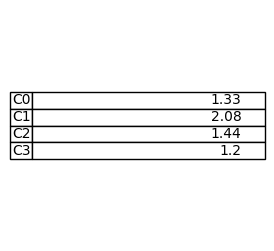
\includegraphics[width=\linewidth]{magnitude2.png}
        \vspace{-2cm}
        \caption{Magnitude of Vectors}
        \label{fig:magnitude}
    \end{minipage}
\end{figure}


Furthermore, adding three more vectors to vector set A and B, to show that, at some point the saturation will occur, the patterns stops recalling perfectly, and the cross-talk increases.

\break

\subsubsection{Adding Three more Vectors}

\begin{table}[ht]
    \begin{center}
        \caption{Vectors \( A \) and \( B \)}
        \begin{tabular}{|c|c|}
            \hline
            \textbf{Input Vector \( A \)} & \textbf{Output Vector \( B \)} \\ \hline
            $[-1, 1, 1, 1, -1]$ & $[1, 1, -1, 1]$ \\ \hline
            $[-1, -1, -1, -1, 1]$ & $[1, -1, -1, -1]$ \\ \hline
            $[-1, -1, -1, 1, 1]$ & $[-1, -1, 1, 1]$ \\ \hline
            $[1, 1, 1, 1, 1]$ & $[-1, 1, 1, -1]$ \\ \hline
            $[-1, -1, 1, -1, -1]$ & $[1, -1, 1, -1]$ \\ \hline
            $[-1, 1, -1, 1, -1]$ & $[-1, -1, -1, -1]$ \\ \hline
            $[1, -1, -1, -1, 1]$ & $[1, 1, -1, -1]$ \\ \hline
        \end{tabular}
    \end{center}
    
\end{table}

The output of the BAM model for the Table 9 Vector input/output pairs is given in Table 10 and Table 11.
Note that, in Table 10, Table 11's most of predicted outputs by the BAM model is false. From A to B output as well as B to A output. This shows that after adding three more vectors in input/output set the model saturated. The models saturates is because of too many similar patterns. Additionally, it could also mean that, there are more overlapping patterns which significantly distorts the output. And the weight matrix saturated at one point hence the model's output is rather inaccurate. Again, from Figure 1.7 shows the original vector set A's magnitude of cross talk, Figure 1.8 shows the magnitude of original vector set plus the given vector pairs in the assignment's magnitude, Figure 1.9 randomly adds three more vectors to the previous vector set. Figure 1.7, 1.8, 1.9 shows the increase in cross talk with more included vector pairs. So, we can conclude that, by adding more vector pairs to the model, it saturates to a point where the model is unable to predict properly. 

\begin{table}[ht]
    \centering
    \caption{Predictions from \( A \) to \( B \)}
    \begin{tabular}{|c|c|c|c|c|}
        \hline
        \textbf{Input \( x \)} & \textbf{Target} & \textbf{Predicted Output \( y \)} & \textbf{Result} \\ \hline
        $[-1, 1, 1, 1, -1]$ & $[1, 1, -1, 1]$ & $[-1, 1, 1, 1]$ & False \\ \hline
        $[-1, -1, -1, -1, 1]$ & $[1, -1, -1, -1]$ & $[1, -1, -1, -1]$ & True \\ \hline
        $[-1, -1, -1, 1, 1]$ & $[-1, -1, 1, 1]$ & $[-1, -1, -1, 1]$ & False \\ \hline
        $[1, 1, 1, 1, 1]$ & $[-1, 1, 1, -1]$ & $[-1, 1, 1, 1]$ & False \\ \hline
        $[-1, -1, 1, -1, -1]$ & $[1, -1, 1, -1]$ & $[1, -1, -1, -1]$ & False \\ \hline
        $[-1, 1, -1, 1, -1]$ & $[-1, -1, -1, -1]$ & $[-1, -1, -1, 1]$ & False \\ \hline
        $[1, -1, -1, -1, 1]$ & $[1, 1, -1, -1]$ & $[1, -1, -1, -1]$ & False \\ \hline
    \end{tabular}
\end{table}

\begin{table}[ht]
    \centering
    \caption{Predictions from \( B \) to \( A \)}
    \begin{tabular}{|c|c|c|c|c|}
        \hline
        \textbf{Output \( y \)} & \textbf{Target} & \textbf{Predicted Output \( x \)} & \textbf{Result} \\ \hline
        $[1, 1, -1, 1]$ & $[-1, 1, 1, 1, -1]$ & $[1, -1, 1, -1, 1]$ & False \\ \hline
        $[1, -1, -1, -1]$ & $[-1, -1, -1, -1, 1]$ & $[-1, -1, -1, -1, -1]$ & False \\ \hline
        $[-1, -1, 1, 1]$ & $[-1, -1, -1, 1, 1]$ & $[-1, 1, -1, 1, -1]$ & False \\ \hline
        $[-1, 1, 1, -1]$ & $[1, 1, 1, 1, 1]$ & $[1, 1, 1, 1, 1]$ & True \\ \hline
        $[1, -1, 1, -1]$ & $[-1, -1, 1, -1, -1]$ & $[-1, -1, -1, -1, -1]$ & False \\ \hline
        $[-1, -1, -1, -1]$ & $[-1, 1, -1, 1, -1]$ & $[-1, -1, -1, -1, -1]$ & False \\ \hline
        $[1, 1, -1, -1]$ & $[1, -1, -1, -1, 1]$ & $[1, -1, 1, -1, 1]$ & False \\ \hline
    \end{tabular}
\end{table}

The cross talk of the following input/output set is provided in Figure 1.5, Figure 1.6. 

\begin{figure}[ht]
    \centering
    \begin{minipage}{0.3\textwidth}
        \centering
        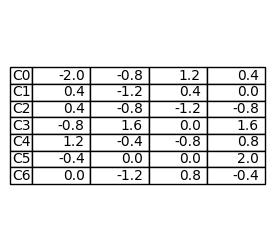
\includegraphics[width=\linewidth]{CrossTalk3.png}
        \vspace{-2cm}
        \caption{Cross Talk of Vectors}
        \label{fig:crosstalk}
    \end{minipage}\hfill
    \begin{minipage}{0.3\textwidth}
        \centering
        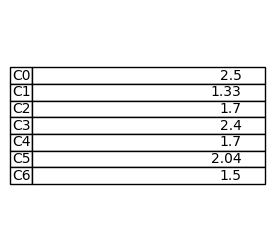
\includegraphics[width=\linewidth]{magnitude3.png}
        \vspace{-2cm}
        \caption{Magnitude of Vectors}
        \label{fig:magnitude}
    \end{minipage}
\end{figure}

\begin{figure}[ht]
    \centering
    \begin{minipage}{0.33\textwidth}
        \centering
        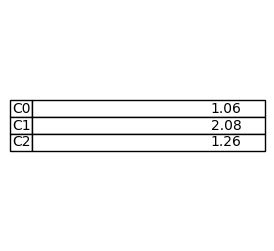
\includegraphics[width=\linewidth]{magnitude.png}
        \vspace{-2cm}
        \caption{Magnitude of Vectors}
        \label{fig:crosstalk}
    \end{minipage}\hfill
    \begin{minipage}{0.33\textwidth}
        \centering
        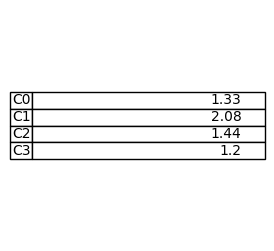
\includegraphics[width=\linewidth]{magnitude2.png}
        \vspace{-2cm}
        \caption{Magnitude of Vectors}
        \label{fig:crosstalk}
    \end{minipage}\hfill
    \begin{minipage}{0.33\textwidth}
        \centering
        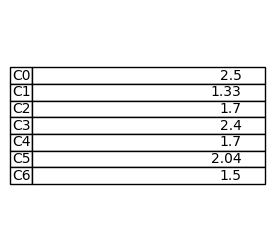
\includegraphics[width=\linewidth]{magnitude3.png}
        \vspace{-2cm}
        \caption{Magnitude of Vectors}
        \label{fig:magnitude}
    \end{minipage}
\end{figure}

\newpage
\clearpage % This will ensure the subsection starts on a new page

\subsection{Part(D)}

In this section, the table is explained in depth. The table contains the 20 recordings of runs, original vector set from Part(A), then a vector is randomly selected to create a mutated vector by flipping the bits, following that, the Hamming distance between original and the mutated vectors, then the mutated vectors were sent through recall function to self correct itself, then hamming distance between original and error corrected is shown, lastly, hamming distance between mutated and error corrected vectors are shown in the table.

\begin{figure}[ht]
    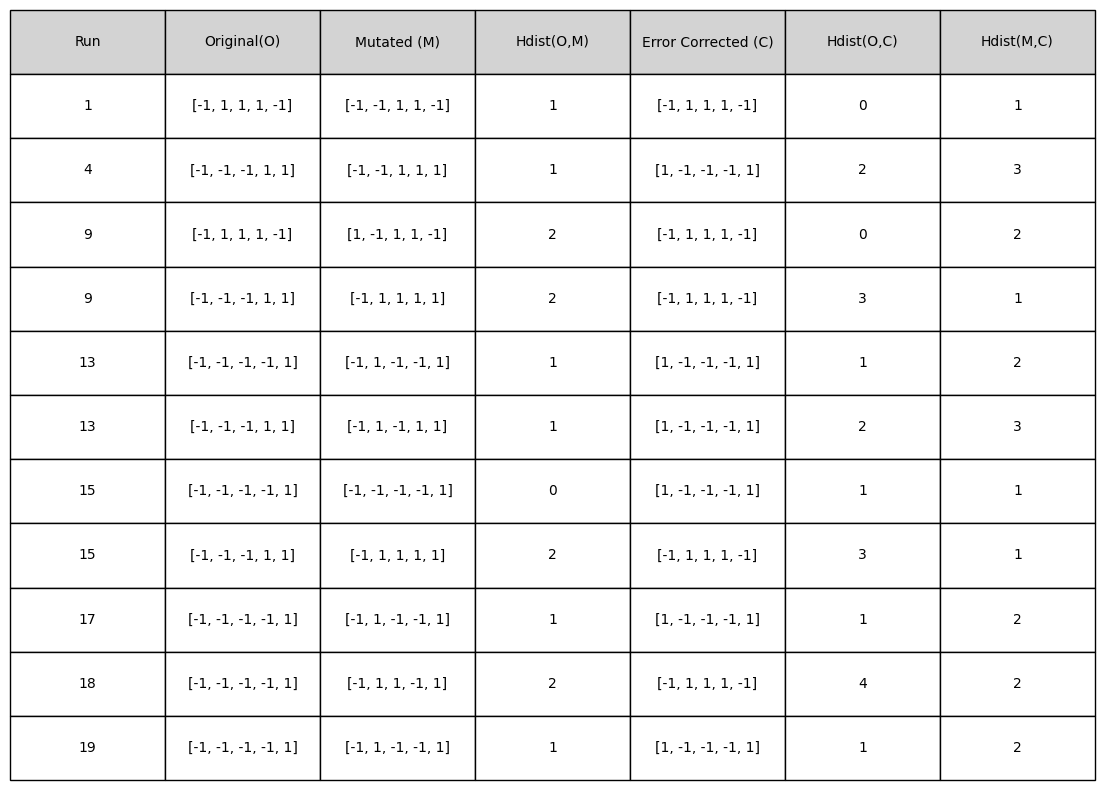
\includegraphics[height=0.5\textheight]{Table.png} % Adjust the height as needed
    \caption{PART D - Table}
    \label{fig:my_image}
\end{figure}

From the table, it is visible that 20 runs were done, however due to mutation rate, the actual run became shorter. Sometimes the program didn't choose to mutate therefore the program terminated if not mutation probability is satisfied. In the mutated section, the mutated vectors differ by 1 bit, since flip bit mutation mechanism was used. Hdist(O,M) shows the hamming distance between original and the mutated vector sets. In the Error Corrected(C) column, the program self corrected the vectors by going 6 times through the recall function for each vector, and tried to get the original vector. From the Hdist(O,C), it shows that sometimes the model is able to correct the mutated vectors, and in some other cases it stays the same. Also, sometimes the model messes the vector while the hamming distance between the original and error corrected vector increases. Only 2 times the model was able to correct the mutated vector properly. While few times the distance between the original and error corrected vectors decreases, few other times it actually increased from the original and mutated distance. The hamming distance between mutated and error corrected sometimes increased by more than 1 bit, or decreased by 1 bit but the model never was able to correctly self correct the mutated input. This is initially because, the model's weight matrix pattern association is limited. Since the model associated the pattern of the initially assigned vectors, it's hard to for the model to predict a mutated vector to it's original form. Futhermore, the memory of BAM model is limited as well.

\subsection{Conclusion}

All the above experiment showed that BAM is a hetero-associative memory. BAM predicts an association B for an input vector A. BAM uses a weight matrix to remember its association with input to output or output to input. BAM is limited, it can only recall the associations properly if the association pattern is stored within the weight matrix. BAM produces cross talk between input and output vectors. The magnitude of the cross talk vector is the interference between the input and output vector. With more inputs, the BAM network increases it's cross talk, meaning the interference. It is possible to error correct a distorted input however, the model has it's limitations.  

\end{document}